% 第8章第1节：初值问题与解（向量场与状态方程；微分形式与积分形式）。

\section{初值问题与解}
\label{sec:ode-ivp}

本节先确定要解的是什么：变化率怎样写成状态方程，高阶方程怎样化成一阶系统，以及一条曲线在什么意义下“满足”方程。存在性和唯一性是下一节的问题；这里只把两件事分开，免得在还不知道解是否存在时就谈论它的性质。

\subsection{向量场与状态方程}
\label{sec:ode-vector-fields}

\paragraph{从变化率到状态方程}
把房间相对室外的温差记作$x(t)$，暖气在时刻$t$送入的加热量记作$u(t)$。温差越大，单位时间散失的热量越多；在最简单的模型里散热率与温差成正比，比例系数$\lambda>0$由墙体和通风决定。于是温差的变化率是补进的热量减去散失的热量：
\begin{equation}
  \dot x(t)=-\lambda x(t)+u(t).
  \label{eq:ode-temperature}
\end{equation}
这里$\dot x$表示对时间的导数。式~\eqref{eq:ode-temperature}没有直接说出$x(t)$等于多少，只说出每个瞬间温差朝哪个方向、以多快的速率变化。本章常取$\lambda=0.2$（时间单位为分钟）和恒定加热量$u=0.4$，这时温差为$2$的状态恰好收支平衡：$-0.2\times2+0.4=0$。

摆给出第二种情形。设摆长为$\ell$，摆角为$\theta$，重力加速度为$g$，空气阻力与角速度成正比，系数为$c\geq0$。牛顿第二定律给出$\ddot\theta=-(g/\ell)\sin\theta-c\dot\theta$。为简化记号，选时间单位使$g/\ell=1$。这个方程含有二阶导数：只知道此刻的角度，还不能决定下一瞬间的变化，因为同一个角度上摆可能正向左摆，也可能正向右摆。

两种情形可以写进同一个框架。把此刻需要知道的量排成状态向量$\bm x(t)\in\mathbb R^d$，把给定的外部作用写成输入$\bm u(t)\in\mathbb R^m$，变化规律写成函数$\bm f$：
\begin{equation}
  \dot{\bm x}(t)=\bm f\bigl(t,\bm x(t),\bm u(t)\bigr),\qquad \bm x(t_0)=\bm x_0.
  \label{eq:ode-ivp-input}
\end{equation}
第一式是状态方程，第二式指定出发的时刻和状态。完整的问题还要说清三样东西：时间在哪个区间$I\ni t_0$中取值；状态允许在哪个开集$D\subseteq\mathbb R^d$中取值，例如浓度只能为正、摆的状态可以取遍$\mathbb R^2$；输入是哪一条事先给定的函数$\bm u:I\to\mathbb R^m$。

本章总把输入当作已经选定的一条时间函数。代入后得到只依赖时间与状态的函数
\[
  \bm g(t,\bm x)=\bm f\bigl(t,\bm x,\bm u(t)\bigr),
\]
状态方程就成为$\dot{\bm x}=\bm g(t,\bm x)$。根据当前状态选择输入，是控制问题要做的事；那时输入本身依赖状态，代入后仍得到一个$\bm g$，但它的性质取决于所选的反馈规则。把“选哪条输入”与“给定输入后怎样求解”分开，本章的结论才能在控制问题中直接使用。

\begin{definition}[初值问题]
  \label{def:ode-ivp}
  设$I\subseteq\mathbb R$是区间，$D\subseteq\mathbb R^d$是开集，$\bm g:I\times D\to\mathbb R^d$，$t_0\in I$，$\bm x_0\in D$。\term{初值问题}（initial value problem）是寻找区间$J\subseteq I$（$t_0\in J$）上的曲线$\bm x:J\to D$，使
  \begin{equation}
    \dot{\bm x}(t)=\bm g\bigl(t,\bm x(t)\bigr),\qquad \bm x(t_0)=\bm x_0.
    \label{eq:ode-ivp}
  \end{equation}
  $\bm g$称为方程的\term{向量场}。“曲线满足方程”的确切含义由定义~\ref{def:ode-classical-solution}和定义~\ref{def:ode-caratheodory-solution}给出。
\end{definition}

方程中只出现状态的一阶导数，因此称为\term{常微分方程}（ordinary differential equation, ODE）；“常”指未知函数只依赖一个自变量$t$。未知量若是依赖时间和空间位置的场，导数就会对多个变量求，得到第~\ref{chap:partial-differential-equations}章的偏微分方程。

\paragraph{斜率场与积分曲线}
在纸上画出向量场，比读公式更容易看出解的样子。对温度模型，在$(t,x)$平面的每个格点上画一小段线段，斜率等于$-0.2x+0.4$。图~\ref{fig:ode-slope-field}(a)显示：温差高于$2$的地方线段向下倾斜，低于$2$的地方向上倾斜，正好在$x=2$处变平。解就是一条处处与这些线段相切的曲线；从不同高度出发的曲线都被线段“引导”向$x=2$靠拢，越靠近越平缓。

\begin{figure*}[htbp]
  \centering
  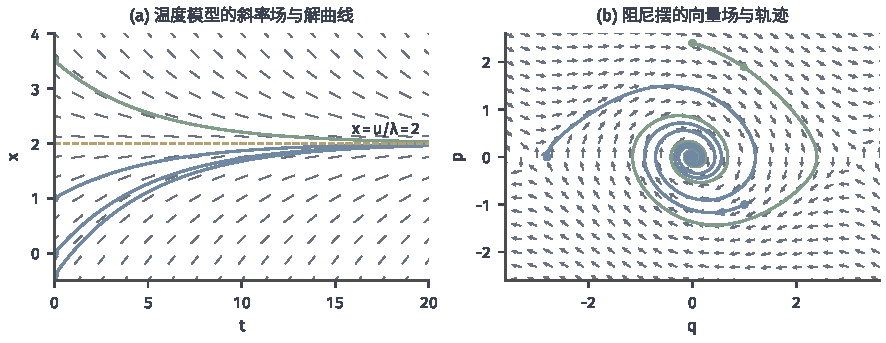
\includegraphics[width=150mm]{figures/03-optimization-evolution-and-signals/02-processes-and-trajectory-evolution/matplotlib/ode-slope-field/figure.pdf}
  \caption{向量场与解曲线。(a)温度模型$\dot x=-0.2x+0.4$的斜率场：每条灰色短线的斜率等于该点的变化率；蓝、绿曲线是从$x_0=-0.4,0,1,3.5$出发的解$x(t)=2+(x_0-2)e^{-0.2t}$，黄色虚线是收支平衡的温差$2$。(b)阻尼摆$\dot q=p$，$\dot p=-\sin q-0.3p$的相平面：箭头只表示向量场方向（已归一化长度），三条轨迹分别从$(-2.8,0)$、$(0,2.4)$、$(1,-1)$出发，计算到$t=25$。}
  \label{fig:ode-slope-field}
\end{figure*}

摆的状态是二维的，可以换一种画法。把角度$q=\theta$和角速度$p=\dot\theta$作为平面坐标，在每一点画出向量$\bigl(p,-\sin q-cp\bigr)$。这个平面称为\term{相平面}，更一般的状态空间也称\term{相空间}（phase space）。图~\ref{fig:ode-slope-field}(b)中，轨迹顺着箭头前进：上半平面$p>0$时角度增大，箭头向右；摆角为正时重力把角速度往下拉，箭头向下。阻尼使每一圈都比上一圈小，轨迹螺旋地落向原点。这里的时间不再是一条坐标轴，而是隐含在沿曲线前进的快慢中；这种画法要求向量场不显含时间，下面马上说明这一点。

\paragraph{高阶方程化为一阶系统}
摆的二阶方程化成了两个一阶方程
\[
  \dot q=p,\qquad \dot p=-\sin q-cp.
\]
做法是把“预测未来需要知道的量”全部放进状态。一般地，若标量未知函数$y$满足$n$阶方程
\[
  y^{(n)}=h\bigl(t,y,\dot y,\ldots,y^{(n-1)}\bigr),
\]
令$x_1=y$，$x_2=\dot y$，……，$x_n=y^{(n-1)}$，就得到一阶系统
\[
  \dot x_1=x_2,\quad\ldots,\quad\dot x_{n-1}=x_n,\quad\dot x_n=h(t,x_1,\ldots,x_n).
\]
相应地，初值必须同时给出$y(t_0),\dot y(t_0),\ldots,y^{(n-1)}(t_0)$这$n$个数。这与第~\ref{chap:discrete-dynamical-systems}章选择离散状态的原则相同：状态要足以决定未来的变化。高阶标量方程与一阶向量系统描述的是同一个对象，只是记号不同；本章的一般理论都对一阶系统陈述。

\paragraph{自治与非自治、线性与非线性}
两组分类经常被混在一起，需要分别说明。若向量场不显含时间，即$\bm g(t,\bm x)=\bm g(\bm x)$，称方程为\term{自治}的（autonomous），否则为非自治的。摆是自治的；温度模型在加热量随时间变化时是非自治的，即使散热系数恒定。自治方程的一个好处正是上面的相平面：同一状态上的方向永远相同，所以可以把方向箭头画在状态空间里而不必记录时间。非自治方程总能通过把时间当作一个新坐标$x_{d+1}=t$、$\dot x_{d+1}=1$改写成自治形式，代价是维数加一。

若$\bm g(t,\bm x)=\bm A(t)\bm x+\bm b(t)$，其中$\bm A(t)\in\mathbb R^{d\times d}$与$\bm b(t)\in\mathbb R^d$只依赖时间，称方程为线性的；$\bm b$不为零时它关于状态其实是仿射的，习惯上仍叫线性方程，$\bm b$称为强迫项。温度模型是线性的，摆因为含$\sin q$而是非线性的。线性与否、自治与否是两项独立的性质：常系数线性系统配上时变输入是线性非自治的，摆是非线性自治的。

\paragraph{与离散更新的对照}
第~\ref{chap:discrete-dynamical-systems}章的一步更新$\bm x_{n+1}=\bm F(\bm x_n)$直接给出下一状态；向量场只给出此刻的瞬时方向。要得到有限时间后的状态，必须沿途把方向累计起来。若在一小段时间$h$内把变化率冻结为起点的值，就得到近似
\[
  \bm x(t+h)\approx\bm x(t)+h\,\bm g\bigl(t,\bm x(t)\bigr).
\]
对温度模型取$h=1$，这个近似是$x(t+1)\approx0.8\,x(t)+u$；而后文第~\ref{sec:ode-constant-linear}小节会算出，在加热量保持不变时，精确的一分钟转移系数是$e^{-0.2}\approx0.8187$。两者接近但不相同，差别来自一分钟之内温差也在变，散热率也随之变化。离散更新与连续方程之间的这种关系，在第~\ref{sec:ode-numerics}节系统讨论。

\subsection{微分形式与积分形式}
\label{sec:ode-integral-form}

\paragraph{经典解与积分方程}
最直接的解的概念是逐点满足方程的可微曲线。

\begin{definition}[经典解]
  \label{def:ode-classical-solution}
  设$\bm g$在$I\times D$上连续。区间$J\ni t_0$上的曲线$\bm x:J\to D$若连续可微，满足$\bm x(t_0)=\bm x_0$，并且$\dot{\bm x}(t)=\bm g(t,\bm x(t))$对每个$t\in J$成立，称为初值问题~\eqref{eq:ode-ivp}的\term{经典解}（classical solution）。
\end{definition}

把方程两边从$t_0$积分到$t$，导数就被换成了状态的增量。这样得到的积分方程不再出现导数，是下一节证明存在唯一性的出发点。

\begin{lemma}[经典解的积分刻画]
  \label{lem:ode-integral-equation}
  设$\bm g$在$I\times D$上连续，$\bm x:J\to D$连续。则$\bm x$是初值问题~\eqref{eq:ode-ivp}的经典解，当且仅当
  \begin{equation}
    \bm x(t)=\bm x_0+\int_{t_0}^t\bm g\bigl(s,\bm x(s)\bigr)\,\mathrm ds\qquad\text{对每个}t\in J.
    \label{eq:ode-integral-equation}
  \end{equation}
\end{lemma}

\begin{proof}
  若$\bm x$是经典解，则$\dot{\bm x}$连续，微积分基本定理给出$\bm x(t)-\bm x(t_0)=\int_{t_0}^t\dot{\bm x}(s)\,\mathrm ds$，再代入方程与初值即得式~\eqref{eq:ode-integral-equation}。反过来，若$\bm x$连续并满足式~\eqref{eq:ode-integral-equation}，则被积函数$s\mapsto\bm g(s,\bm x(s))$是连续函数的复合，因而连续；微积分基本定理说明右端关于$t$连续可微，导数等于$\bm g(t,\bm x(t))$。于是$\bm x$连续可微并满足方程，代入$t=t_0$得到初值。
\end{proof}

式~\eqref{eq:ode-integral-equation}有一个直观的读法：此刻的状态等于出发时的状态，加上一路上速度的累计。对标量方程，它就是“初值加上速度曲线下的面积”。这个读法把求解问题变成了一个自洽条件：曲线$\bm x$决定了沿途的速度$\bm g(s,\bm x(s))$，速度的累计又必须重新给出同一条曲线。

\paragraph{只可测的输入}
经典解要求$\bm g$关于时间连续，实际的输入却常常有跳变。设暖气在前$5$分钟以$u=0.4$加热，随后关闭，即
\[
  u(t)=\begin{cases}0.4,&0\leq t<5,\\0,&t\geq5.\end{cases}
\]
在$t=5$处方程右端跳变，任何可微曲线都无法在这一点同时满足左右两侧的方程。但积分方程~\eqref{eq:ode-integral-equation}对这种分段常值输入仍然有意义，而且房间的温度在物理上确实随时间连续变化。

\begin{example}[开关暖气下的温差]
  \label{ex:ode-switched-heating}
  取$\lambda=0.2$，$x(0)=0$，输入如上。在$[0,5]$上，$x(t)=2(1-e^{-0.2t})$，于是$x(5)=2(1-e^{-1})\approx1.2642$。$t\geq5$时只剩散热，从这个值出发得到$x(t)=1.2642\,e^{-0.2(t-5)}$。两段在$t=5$处连在一起，但左导数$-0.2\times1.2642+0.4\approx0.1472$与右导数$-0.2\times1.2642\approx-0.2528$不同，曲线在这里出现折角。直接验算可知，这条曲线对每个$t\geq0$都满足积分方程~\eqref{eq:ode-integral-equation}，并且除$t=5$外处处满足微分方程。
\end{example}

这个例子提示应当放宽解的概念：允许在一个“可以忽略”的时刻集合上不可导，只要积分关系成立。可是放宽到什么程度？仅要求曲线连续、几乎处处满足方程是不够的。Cantor函数$c:[0,1]\to[0,1]$连续、单调不减，在Cantor集之外导数为零，而Cantor集的Lebesgue测度为零；可它从$c(0)=0$升到$c(1)=1$，并不是常数。若只要求几乎处处满足方程，Cantor函数就会成为方程$\dot x=0$、$x(0)=0$的一个“解”，零解的唯一性也就无从谈起。问题在于Cantor函数的全部变化都藏在导数看不见的零测集上，不能由导数积分还原。

能够由导数积分还原的函数恰好是绝对连续函数：若$x$在$[a,b]$上绝对连续，则它几乎处处可导，导数可积，并且$x(t)=x(a)+\int_a^t\dot x(s)\,\mathrm ds$；反之，可积函数的不定积分总是绝对连续的。这一刻画及Cantor函数为什么不绝对连续，可参考\BookChapterRef{chap:integration}{卷二“积分”章}。向量值曲线按分量理解，于是得到下面的定义。

\begin{definition}[绝对连续曲线]
  \label{def:ode-absolutely-continuous-curve}
  有限闭区间$[a,b]$上的曲线$\bm x:[a,b]\to\mathbb R^d$称为\term{绝对连续曲线}，若存在可积函数$\bm v\in L^1([a,b];\mathbb R^d)$，使$\bm x(t)=\bm x(a)+\int_a^t\bm v(s)\,\mathrm ds$对每个$t\in[a,b]$成立。此时$\dot{\bm x}=\bm v$几乎处处成立。一般区间上的曲线若在其中每个有限闭子区间上绝对连续，称为局部绝对连续。
\end{definition}

为让积分方程中的被积函数可积，需要对$\bm g$加下面三条要求，它们合称为\term{Carathéodory条件}：
\begin{enumerate}
  \item 对每个固定的$\bm x\in D$，$t\mapsto\bm g(t,\bm x)$可测；
  \item 对几乎每个$t\in I$，$\bm x\mapsto\bm g(t,\bm x)$连续；
  \item 对每个紧集$K\subseteq D$，存在在$I$的每个有限闭子区间上可积的函数$m_K\geq0$，使$\|\bm g(t,\bm x)\|_2\leq m_K(t)$对几乎每个$t$与全部$\bm x\in K$成立。
\end{enumerate}
前两条保证对每条连续曲线$\bm x$，复合函数$s\mapsto\bm g(s,\bm x(s))$可测；第三条保证当曲线留在紧集$K$中时，这个复合函数可积。若$\bm f$关于$(t,\bm x,\bm u)$连续，输入$\bm u$可测且局部有界，则$\bm g(t,\bm x)=\bm f(t,\bm x,\bm u(t))$满足这三条：第三条中的上界可取为$\bm f$在一个紧集上的最大值。开关暖气的例子正是这种情形。

\begin{definition}[Carathéodory解]
  \label{def:ode-caratheodory-solution}
  设$\bm g$满足Carathéodory条件。区间$J\ni t_0$上局部绝对连续的曲线$\bm x:J\to D$，若对每个$t\in J$满足积分方程~\eqref{eq:ode-integral-equation}，称为初值问题的\term{Carathéodory解}。等价地，$\bm x(t_0)=\bm x_0$且$\dot{\bm x}(t)=\bm g(t,\bm x(t))$对几乎每个$t\in J$成立。
\end{definition}

两种表述等价，正是绝对连续曲线的作用：积分方程给出的曲线自动绝对连续并几乎处处满足方程；反过来，一条几乎处处满足方程的绝对连续曲线可以由导数积分还原，因而满足积分方程。当$\bm g$连续时，引理~\ref{lem:ode-integral-equation}说明Carathéodory解就是经典解，所以这是对经典概念的推广而不是替换。本章在$\bm g$连续时直接说“解”指经典解；输入只可测时说“解”指Carathéodory解。

\paragraph{满足方程与解的存在是两个问题}
到这里只回答了“什么样的曲线算解”，还没有回答“这样的曲线是否存在、有几条、能延续多久”。积分方程~\eqref{eq:ode-integral-equation}把后一组问题变成了一个不动点问题：在曲线组成的集合上，映射
\[
  \bm x\longmapsto\bm x_0+\int_{t_0}^{\cdot}\bm g\bigl(s,\bm x(s)\bigr)\,\mathrm ds
\]
把一条候选曲线送到另一条曲线，解就是被送回自身的曲线。下一节研究这个映射在什么条件下恰有一个不动点。
